
\chapter{Avionics}
\section{Requirements}
The avionics subteam is responsible for completion of a multitude of critical objectives. Specifically, the avionics team was charged with the following: first, the team is responsible for transmitting the deployment signal to the \gls{uav} after receiving clearance from the \gls{rso} so that the rocket’s payload can be ejected. Moreover, the team must know the exact altitude of the rocket through the use of a commercially available altimeter.
Furthermore, the avionics subteam is also responsible for triggering the e-matches which then deploy the main and drogue parachutes
at the correct point in the flight. This is of critical importance to the success of the mission because these signals are used to deploy the parachutes at the correct moment for landing.
In addition to satisfying these team defined objectives, the team must also design the avionics system pursuant to the requirements of the competition as specified in the NASA Student Launch handbook. The following section establishes the aforementioned requirements and the team’s efforts to meet them. 

The first critical requirement that falls on the avionics team concerns the barometric altimeter. The rocket must include one commercially available barometric altimeter. The team will include the MPL3115A2 by Xtrinsic, a commercially available altimeter as part of the avionic subsystem for the rocket. 
In addition to the commercially available barometric altimeter mentioned above, there are two other sets of altimeters deployed in a two-pairs-of-two configuration that provides quadruple redundancy. In total, there will be five Altimeters. The first two is the PrefectFlite Stratologger and the other two altimeters we will be using is the Atlus Metrum TeleMetrum. They will be configured in two sets of both altimeters on the rocket. The avionics subteam focused on adding redundancy in the altimeter configuration. As mentioned earlier, there are four altimeters in addition to the  MPL3115A2. The TeleMetrum altimeter will serve as the backup altimeter in each pair to the Stratologger. Moreover, each altimeter will act as a fully self-contained system, with its own source of power (via a battery). Additionally, each altimeter will be armed via a dedicated arming switch that can be accessed from the exterior of the rocket frame. Each arming switch individually locks in its on position once set by a team member; this prevents it from getting disarmed by forces present in flight. Moreover, lithium polymer batteries will be clearly indicated as a fire hazard to ensure safety. All the electronics, including LiPo batteries will be physically segregated from the payload to prevent any damage during the payload deployment. Furthermore, in order to prevent the batteries from being damaged during flight, they will be mounted to a fixed part of the interior of the rocket. 
The TeleMetrum has an onboard GPS receiver which will be able to keep track of the rocket’s position. This will allow the team to easily recover the rocket. Additionally, the team is strongly considering adding additional GPS sensors to the rocket in order to give the ground receiver a more accurate estimation of the rocket’s position. All rocket sections, which are untethered to the fuselage, including the payload, will contain separate tracking devices as well. The team plans to thoroughly test the avionics of the rocket to ensure that all tracking devices will be fully functional on launch day.
In addition to the altimeters and recovery devices, in order to deploy the payload, we will be using an XBee Pro S3B RF module. The Xbee Pro can operate on a multitude of channels between 900.0 MHz and 928.0 MHz, ensuring that channel conflicts can be accommodated by altering the channel. The avionics components must be continuously powered for 2 hours on the launch site without losing its functionality, which will be accomplished by having a power capability that can account for the power consumption of the important on-board electronics. The estimated run time is detailed in a table below.
The team also plans to shield the on-board electronic components in order to lower the risk of failure of these systems. The team will ensure that the altimeters will be isolated from any electromagnetic interference producing devices to prevent damage or other interference with the of the recovery system. Moreover, the team will have to use adequate shielding to prevent the recovery system from being unexpected excitation of the system.

\section{Design Considerations}

In order to fulfill the aforementioned requirements and ensure mission success. The team investigated component selection and other design considerations. The first element of the avionics deployment was the control board that functions as the processing unit behind the system.
The control board for telemetry and UAV Aerial Deployment System will play a critical importance. ISS has had prior success with the Arduino microcontroller, but the Raspberry Pi was also considered as it provided greater processing power and increased control. The trade-off between the two systems was carefully considered as it constituted a major design decision. 
	The Arduino was initially considered because it has a proven track record with ISS. It’s simplicity and ease-of-use provides the team with flexibility, and there is a vibrant online community that through the use of forums and other educational websites provides guidance and support to other users of the Arduino development platform. Moreover, Arduino is easier to understand and program as it uses a modified version of C++, which is a common programming language, in a native, self-contained integrated development environment (IDE) known as the Arduino IDE. 
	There are multiple versions of the Arduino platform. One mode of variation is the size of the Arduino module. In particular, two versions of the Arduino platform with through-hole mounting capability that were considered were the Arduino Micro and Arduino Nano. The two are similar in size and mass with the latter being slightly smaller (48mm vs 45mm, respectively) and lighter (13g vs 7g). The critical difference was the power delivery capability between the two platforms. The Arduino Nano is capable of delivering twice the current per pin at 40 mA compared to the Micro’s limitation of 20 mA, with the recommended current draw being half the maximum. This limitation would severely limit the team’s ability to power additional components with the Arduino’s regulated 5 and 3.3 volt supply rails, which would require that additional circuitry be introduced to power the components. It was therefore, decided that the Arduino Nano would be the Arduino of choice. The Raspberry Pi was also considered as an alternative. \\\\
The Raspberry Pi is a flexible, general purpose computer with exponentially higher processing power and memory capacity than the Arduino. However, the Raspberry Pi’s additional power and multi-platform support means that the implementation of the requisite functionality would be harder and expose the team to a greater risk of software related errors. The team therefore considered if the Arduino processing capabilities would be sufficient for the telemetry and data logging needs. 
	The functionality required from the micro-controller essentially remains unchanged from the proposal. It is required to control and preferably power the communication system and additional data logging system. These requirements can be reasonably met and exceeded by both platforms. Therefore, the Arduino was selected as the team was more experienced with the platform. 
The team initially wanted to incorporate an Inertial Measurement Unit (IMU) in the sensor deployment as it would provide useful data about the rocket in flight. The IMU measures linear and rotational accelerations and this data is logged to onboard storage. The team had multiple IMUs on hand. The LSM9D51 by iNEMO was the most fully featured IMU owned by the team. Because ISS has had prior success using this unit, the team was actively considering it. In addition to the LSM9D51, the team also considered purchasing a new IMU, the BOSCH BNO055. The conclusion, which will be explored in greater detail in the following paragraphs, are as follows: the BNO055 does not warrant purchase as its expanded feature set does not justify the financial cost and risk of deploying a new component.  
From a functional perspective, the LSM9D51 and the BNO055 had an accelerometer, a gyroscope, and a magnetometer and can therefore read similar sensor data. In terms of data transfer protocols, the BNO055 supports the (Inter-Integrated Circuit) I2C protocol, while the LSM9D51 can also support the Serial Peripheral Interface protocol. This did not significantly influence the selection of IMU as the I2C is far more versatile as it doesn’t require separate chip select lines, and its lower data transfer rates and half-duplex nature is of little importance to the overall functionality of an IMU that does not require significant bandwidth.\\\\
The electrical specifications of the two IMUs are similar. Both the LSM9D51 and BNO055 have a normal operating mode and a low power mode. They also both can tolerate a range of driving voltages, and the regulated 3.3V output of the Arduino falls in both ranges. However, according to the datasheets, the current draw of the LSM9D51 under the normal operating mode is around 4.6 mA, therefore the power consumption of LSM9D51 is approximately 15.18mW. For the BNO055, the current draw is \SI{12.3}{\milli\ampere}, resulting in an estimated power consumption of 40.59 mW. This has the following implications: firstly, the system can run for a significantly longer time on battery power when using the LSM95D1 as opposed to the BNO055. Secondly, the Arduino Nano has a package current limit of 200 mA. Therefore, by using the LSM9D51 instead of the BNO055, additional sensors can be deployed without approaching the upper limit of the specification. 	
A key component for a successful deployment of the UAV, being critical to the success of the mission, is a barometric altimeter. In order to deploy the payload, two signals are needed. The first is the signal from the range safety officer indicating it is safe to deploy. The second signal we need is a ready signal from the altimeter indicating that the rocket is at the correct altitude for deploying the payload. Therefore, the team decided to deploy a barometric altimeter in addition to the IMU. 
	The barometric altimeter that the team will be using for this mission is the MPL3115A2  by Xtrinsic. This sensor can measure barometric pressure, temperature and altitude. This sensor is of critical importance to the team because the deployment of the payload must happen at a specified altitude. This altimeter needs a supply voltage of between 1.95 and 3.6 volts. The maximum current of the altimeter is 2mA, but  when the sensor is in standard operating modes, it can draw a max of \SI{265}{\micro\ampere}. There are two primary power modes for this altimeter. The first power mode is the standby mode. In standby mode digital sections are operational and the unit is capable of receiving commands and delivering stored data. Finally, there is the active mode. In this mode the system is fully functioning with both the analog and digital sections running. 
Two RF systems the team considered for use in this mission were the HC-12 wireless transceiver module and the XBee Pro S3B RF Module. The first design consideration of these sensors the team had to consider was the range. While the claimed range of the XBee Pro is far superior to that of the HC-12, and the XBee Pro also has significantly more bandwidth at 230400 baud compared to the 115,600 baud. The working frequency of the XBee Pro is double that of the HC-12 (900 MHz vs 430 MHz, respectively). Moreover, using the XBee Pro  would result in losing the benefit of experience with the HC-12. However, the impact of this is ameliorated by the XBeePro’s far superior documentation. This would enable the team to  compensate for the lack of experience with the device.

Regarding power, the Arduino is the primary source of power for the communication modules. Therefore, the current draw of the communication modules must be compatible with what the Arduino can provide, which is 200 mA in total, 20 mA suggested per pin, and a maximum of 40 mA per pin. For the HC-12, the power delivery capabilities on an Arduino is adequate. However, the XBee Pro, which draws 55 - \SI{215}{\milli\ampere} at \SI{3.3}{\volt}, uses much more power than the HC-12, which draws \SI{16}{\milli\ampere} at its high power mode. To account for the additional power needs of the XBee Pro, the team would have to connect to the battery through a voltage regulator capable of supplying the needed current. The avionics system will also be powering the winch system's servo of the UAV deployment system. This will be powered from the Arduino's power system. The current draw of the servo will be tested and if it is found to draw too much current from the Arduino, the team will use a darlington transistor to control the servo. Moreover, a flyback diode will be used to prevent back-EMF spikes. The team began by performing range tests between two HC-12 modules.
Upon performing range tests for the HC-12 unit, the team found it unsuitable for use in a mission involving rockets and long-range communication. Firstly, a circuit was constructed using two breadboards, two HC-12, and two Arduino UNO R3s. One HC-12 was programmed using the Arduino IDE to transmit a string of bits continuously while the other HC-12 would continuously receive this message. The test involved having one HC-12 unit being held stationary and the other was moved by a team member along a long and straight street. The objective of this test was to determine when exactly the transmitting HC-12 was out of range of the receiving HC-12. The test showed that the HC-12 began dropping packets of data at an estimated \SI{60}{\meter}. The test also showed that the message did not come through fully and would often get distorted by errors.
\\\\
Therefore, the team concluded that the HC-12 should not be used by our team for this mission. Instead the team should use the XBee Pro unit due to its superior range and bandwidth, along with a necessary driving circuit required to fully accommodate this unit. A similar testing procedure will be applied to the Xbee Pro module to validate its performance and reliability.
The remaining avionics system concerns itself with successful deployment of the main and drogue parachutes. The StratoLogger will serve as the rocket’s primary altimeter. The module will enable the team to capture critical data about the flight’s altitude, profile, and velocity. It will be powered by a nine-volt commercially available battery. This power system will function in tandem with the StratoLogger’s own brownout protection system which can power the device for two seconds after a brownout, or unexpected voltage drop or power loss, occurs. The StratoLogger's duty as the primary altimeter means that it will control the e-matches charged with deploying the drogue and main parachutes when pre-set altitudes are reached. The StratoLogger will be manually enabled by an arming switch that is accessible from the exterior of the fuselage. This will mitigate risk associated with premature triggering of the black powder charges. The StratoLogger has a working range of upto 100,000 feet MSL. The module’s storied history a part of ISS’ avionics deployment also re-assures the team that a critical component for the safety and success of the mission will work function as required. Two Stratologgers will be deployed consistent with the proposal to ensure redundancy. 
In order to provide additional redundancy, the team decided to include two TeleMetrums as the secondary altimeters on the rocket. The dual deployment configuration features the TeleMetrum as backup altimeter in an altimeter pair. Therefore, it is responsible for secondary control over the two charges responsible for deploying the main and drogue parachutes in the case of a failure in the primary system (Stratologger). The Telemterum comes with an integrated GPS receiver along with barometric pressure sensors that are rated up to 100,000 feet MSL. Additionally, the TeleMetrum modules are powered by a 900 mAh \SI{3.7}{\volt} LiPo battery and the voltage on battery will be verified prior to the launch to ensure full capacity. Finally, since the GPS receiver on the TeleMetrum can function as a tracking beacon, it will be used during the rocket recovery. 
	The team will prepare a preliminary avionics system complete with the UAV deployment signal transceivers and quadruply redundant altimeter configuration. The system will help the team analyze the performance of the rocket during its subscale flight. Moreover, the flight will help tailor the sensor and telemetry deployment. The team also is investigating the use of printed circuit oards (PCB), and both surface mount components (SMT) and through-hole components. The use of a PCB helps mitigate risk of damage to the circuit due to mechanical stresses, at little additional cost.

\begin{table}[H]
    \centering
    \caption{Avionics Current Consumption At Nominal Voltage}
    \label{tab:Avionics:PowerConsumption}
    \begin{tabularx}{\linewidth}{X X X X}
        \toprule
        \textbf{Device} & \textbf{Current Consumption} & \textbf{Estimated Battery Size} & \textbf{Estimated Run Time \newline Exceeds 2 Hours} \\
        \midrule
        Stratologger & Typical: \SI{1.5}{\milli\ampere},\newline Firing: 5 A & \SI{500}{\milli\ampere\hour} & \cmark \\ \\
        Telemetrum & 60 - \SI{80}{\milli\ampere} & \SI{900}{\milli\ampere\hour} & \cmark
        \\ \\
        Xbee Pro & \SI{215}{\milli\ampere} & \SI{1200}{\milli\ampere\hour} & \cmark \\ \\
        Arduino Nano & \SI{200}{\milli\ampere} & \SI{1200}{\milli\ampere\hour} & \cmark \\
        \bottomrule
    \end{tabularx}
\end{table}

\begin{figure}[H]
    \begin{subfigure}[b]{.49\linewidth}
        \centering
        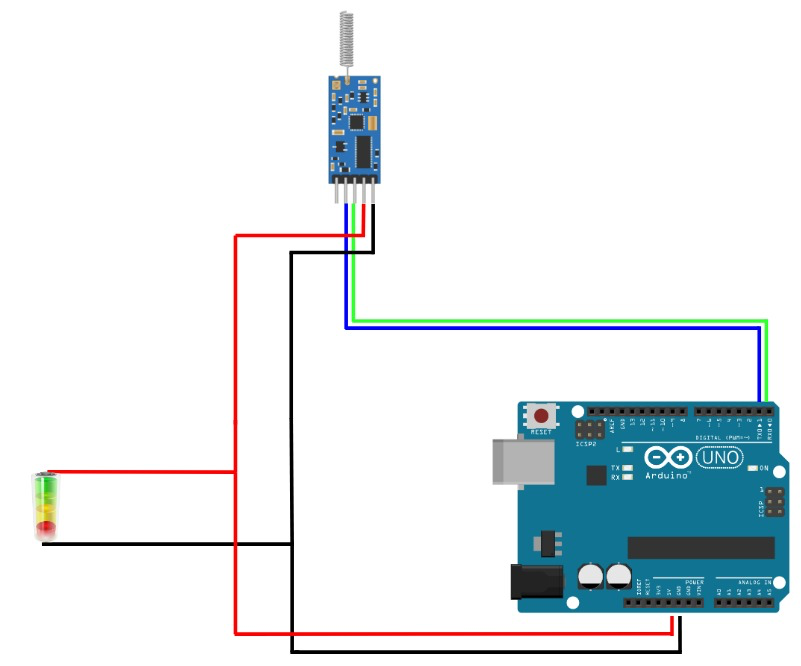
\includegraphics[width=\linewidth]{img/AV/HC12.jpg}
        \label{HC-12schematics}
        \caption{HC-12 schematic}
    \end{subfigure}
    \begin{subfigure}[b]{.49\linewidth}
        \centering
        \includegraphics[width=\linewidth]{img/AV/StratoLogger.png}
        \caption{Stratologger Wiring Block Diagram}
    \end{subfigure}
    \caption{(a) HC-12 and Arduino Configuration with External Power, (b) Stratologger Block Diagram}
\end{figure}

  \begin{table}[htbp]
    \centering
    \caption{Failure Modes and Risk Analysis}
    \begin{tabularx}{\linewidth}{X >{\centering\arraybackslash}m{1in} X}
    \toprule
    \textbf{Failure Modes} & \textbf{RAC} & \textbf{Mitigation approach} \\
    \midrule
    \renewcommand{\arraystretch}{1.5}%
    \ E-match system failure & \cellcolor{green!25} \textbf{\newline \newline 1E} 
  & Risk is minimized by using ematches in a fully redundant system. \\
  Either parachute deploys prematurely in flight & \cellcolor{green!25}\textbf{\newline \newline \newline 2E} & The deployment system will be tested prior to launch, and feature reliable components.  \\
  Either parachute deploys prematurely on launch pad & \cellcolor{green!25}\textbf{\newline \newline \newline 1E} & A mechanical arming switch will be installed that interrupts the system's access to power to ensure that the black powder charges deploy.  \\
  Altimeter brown or black-out & \cellcolor{orange!25}\textbf{\newline \newline \newline \newline 2D} & The system will be designed to be tolerant to power loss. Specifically, the stratologger was selected because of its two second brown out protection. \\
  Communications failure & \cellcolor{orange!25}\textbf{\newline \newline \newline \newline \newline 3C} & The communication system will use commericially available radios with specifications that far exceed the required range and throughput. The system will be shielded against electromagnetic interference, and the radios will operate on clear channels. \\
  Short circuit in the avionics system & \cellcolor{green!25}\textbf{\newline \newline 3D} & The team will perform exahustive testing of avionics systems before use in rocket. The team will also use multimeters to check for short circuits or ground faults.  \\
  Battery failure (excluding altimeters) & \cellcolor{orange!25}\textbf{\newline \newline  \newline \newline  1D} & The team will use a multimeter to inspect the batteries and additional testing of the avionics systems before final use. The batteries will be sized appropriately with a large tolerance to ensure that launch delays do not impact the rocket. \\
  Disconnection of soldered connections, caused by flight and launch forces. & \cellcolor{orange!25}\textbf{\newline \newline \newline 3C} & The team will ensure that solder joints are secured, and is investigating the use of a PCB which would strongly mitigate the risk. \\

      \bottomrule
      \end{tabularx}%
    \label{tab:addlabel}%
  \end{table}%

  


